%
%Projekt:	ITY 3.projekt 
%Autor:		Peter Tisovcik - xtisov00@stud.fit.vutbr.cz
%Datum:		01.04.2015
%
\documentclass[11pt, a4paper, titlepage] {article} 
    \usepackage[left=2cm, text={17cm, 24cm}, top=3cm ]{geometry}  
    \usepackage[czech]{babel}
	\usepackage[utf8]{inputenc}
	\usepackage{times} 
	\usepackage[T1]{fontenc}
	\usepackage{multirow}
	\usepackage[ruled, longend,czech, linesnumbered, noline]{algorithm2e}
	\usepackage{graphicx}
	\usepackage{graphics}
	\usepackage{picture}
	\usepackage{epstopdf}
	\newcommand{\myuv}[1]{\quotedblbase #1\textquotedblleft}
	
\begin{document}

%%%%% Title page 
\begin{titlepage}
\begin{center}
	{\Huge\textsc{Vysoké učení technické v~Brně}}\\
\medskip
{\huge\textsc{Fakulta informačních technologií}}\\
\vspace{\stretch{0.382}}
{\LARGE Typografie a~publikování\,--\,3.\,projekt}\\
\medskip
{\Huge Tabulky a~obrázky}\\
\vspace{\stretch{0.618}}
\end{center}
{\LARGE \today \hfill Peter Tisovčík}
\end{titlepage}
	
\section{Úvodní strana}
Název práce umístěte do zlatého řezu a~nezapomeňte uvést dnešní datum a~vaše jméno a~příjmení.

\section{Tabulky}
Pro sázení tabulek můžeme použít buď prostředí \texttt{ tabbing } nebo prostředí \texttt{ tabular}.

\subsection{Prostředí \texttt{ tabbing}}
Při použití \verb| tabbing | vypadá tabulka následovně:

\begin{tabbing}
	Vodní melouny \quad\= \textbf{Cena} \quad\= \textbf{Množství} \kill
	\textbf{Ovoce} \> \textbf{Cena} \> \textbf{Množství}\\
	Jablka \> 25,90 \> 3\,kg\\
	Hrušky \> 27,40 \> 2,5\,kg\\
	Vodní melouny \> 35,-- \> 1\,kus
	\\
\end{tabbing}
Toto prostředí se dá také použít pro sázení algoritmů, ovšem vhodnější je použít prostředí \texttt{ algorithm } nebo \texttt{algorithm2e} (viz sekce \ref{algoritmy}).

\subsection{Prostředí \texttt{ tabular}}
Další možností, jak vytvořit tabulku, je použít prostředí \texttt{ tabular}. Tabulky pak budou vypadat takto\footnote{Kdyby byl problém s\texttt{ cline, }zkuste se podívat třeba sem:
http://www.abclinuxu.cz/tex/poradna/show/325037.}:


\begin{table}[h]  
\begin{center}
\catcode`\-=12 %nastavenie spraveho prekladu pre -
\begin{tabular}{| c | r | r |} 
	\hline &
    \multicolumn{2}{|c|}{\textbf{Cena}}\\ \cline{2-3}
    \textbf{Měna} & \textbf{nákup} & \textbf{prodej}\\ \hline
    EUR & 27,34 & 27,42\\
    GBP & 33,09 & 33,21\\
    USD & 19,87 & 19,95\\ \hline
\end{tabular}
\caption{Tabulka kurzů k~dnešnímu dni}
\label{kurzy}
\end{center}
\end{table}





\begin{table}[h]
\begin{center}
\catcode`\-=12 %nastavenie spraveho prekladu pre -
\begin{tabular}{|c|c|}
	\hline
	$A$ & $\neg A$\\ \hline
	\textbf{P} & N\\ \hline
	\textbf{O} & O\\ \hline
	\textbf{X} & X\\ \hline
	\textbf{N} & P\\ \hline
\end{tabular}
\begin{tabular}{|c|c|c|c|c|c|}
	\hline
	\multicolumn{2}{|c|}{\multirow{2}{*}{$A\wedge B$}} & \multicolumn{4}{c|}{$B$}\\ \cline{3-6}
    \multicolumn{2}{|c|}{} &\textbf{P} & \textbf{O} & \textbf{X}& \textbf{N} \\ \hline
    \multirow{4}{*}{$A$} & \textbf{P} & P & O & X & N \\ \cline{2-6}
    & \textbf{O} & O & O & N & N \\ \cline{2-6}
    & \textbf{X} & X & N & X & N \\ \cline{2-6}
    & \textbf{N} & N & N & N & N \\ \hline
\end{tabular}
\begin{tabular}{|c|c|c|c|c|c|}
	\hline
	\multicolumn{2}{|c|}{\multirow{2}{*}{$A\vee B$}} & \multicolumn{4}{c|}{$B$}\\ \cline{3-6}
    \multicolumn{2}{|c|}{} &\textbf{P} & \textbf{O} & \textbf{X}& \textbf{N} \\ \hline
    \multirow{4}{*}{$A$} & \textbf{P} & P & P & P & P \\ \cline{2-6}
    & \textbf{O} & P & O & P & O \\ \cline{2-6}
    & \textbf{X} & P & P & X & X \\ \cline{2-6}
    & \textbf{N} & P & O & X & N \\ \hline
\end{tabular}
\begin{tabular}{|c|c|c|c|c|c|}
	\hline
	\multicolumn{2}{|c|}{\multirow{2}{*}{$A\rightarrow B$}} & \multicolumn{4}{c|}{$B$}\\ \cline{3-6}
    \multicolumn{2}{|c|}{} &\textbf{P} & \textbf{O} & \textbf{X}& \textbf{N} \\ \hline
    \multirow{4}{*}{$A$} & \textbf{P} & P & O & X & N \\ \cline{2-6}
    & \textbf{O} & P & O & P & O \\ \cline{2-6}
    & \textbf{X} & P & P & X & X \\ \cline{2-6}
    & \textbf{N} & P & P & P & P \\ \hline
\end{tabular}
\caption{Protože Kleeneho trojhodnotová logika už je
\label{tabulky} \myuv{zastaralá}, uvádíme si zde příklad čtyřhodnotové logiky}
\end{center}
\end{table}


\section{Algoritmy}\label{algoritmy}
Pokud budeme chtít vysázet algoritmus, můžeme použít prostředí \texttt{algorithm\footnote{Pro nápovědu, jak zachádet s~prostředím \texttt{ algorithm, } můžeme zkusit tuhle stránku:\\http://ftp.cstug.cz/pub/tex/CTAN/macros/latex/contrib/algorithms/algorithms.pdf.} } nebo \texttt{ algorithm2e}\footnote{Pro \texttt{ algorithm2e } zase tuhle: http://ftp.cstug.cz/pub/tex/CTAN/macros/latex/contrib/algorithm2e/doc/algorithm2e.pdf.}. Příklad použití prostředí \texttt{ algorithm2e } viz Algoritmus \ref{algoritmus-1}.

\bigskip
\begin{algorithm}
\SetNlSty{}{}{:} %dvojbodka za cislami riadkov
\KwIn {$(X_{t-1}, u_{t}, z_{t})$} 
\KwOut{$X_t$}
\BlankLine
\SetNlSkip{-1.2em}
\Indp
$\overline{X_t} = X_t = 0$\\  
\For{$k=1$ \KwTo $M$}
{	$x_t^{[k]}=sample\_motion\_model(u_t, x_{t-1}^{[k]})$\\
	$w_t^{[k]}=measurement\_model(z_t, x_t^{[k]}, m_{t-1})$\\
	$m_t^{[k]}=updated\_occupancy\_grid(z_t,  x_t^{[k]}, m_{t-1}^{[k]})$\\
	$\overline{X_t} = \overline{X_t}\,+\,\langle x_x^{[m]}, w_t^{[m]}\rangle$\\
}
\For{$k=1$ \KwTo $M$}
{	draw $i$ with probability $\approx w_t^{[i]}$\\
	add  $\langle x_x^{[k]}, m_t^{[k]}\rangle$ to $X_t$
}
\Return{$X_t$}
\caption{\textsc{Fast}SLAM \label{algoritmus-1}}
\end{algorithm}

\section{Obrázky}
Do našich článků můžeme samozřejmě vkládat obrázky. Pokud je obrázkem fotografie, můžeme klidně použít bitmapový soubor. Pokud by to ale mělo být nějaké schéma nebo něco podobného, je dobrým zvykem takovýto obrázek vytvořit vektorově.

\begin{figure}[ht]
\begin{center}
\scalebox{0.37}
{	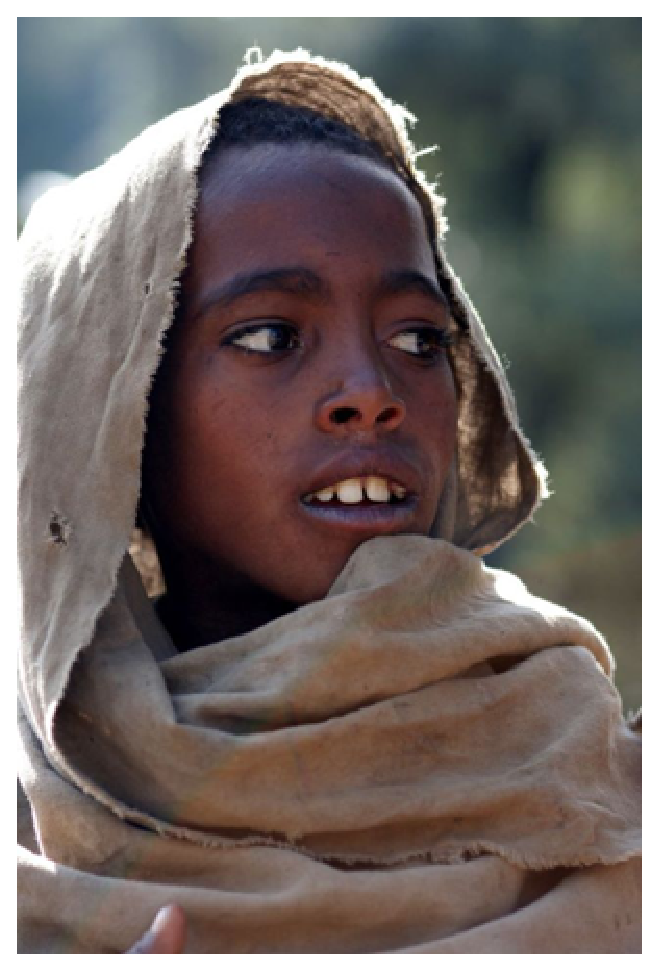
\includegraphics{etiopan.eps}
	\reflectbox{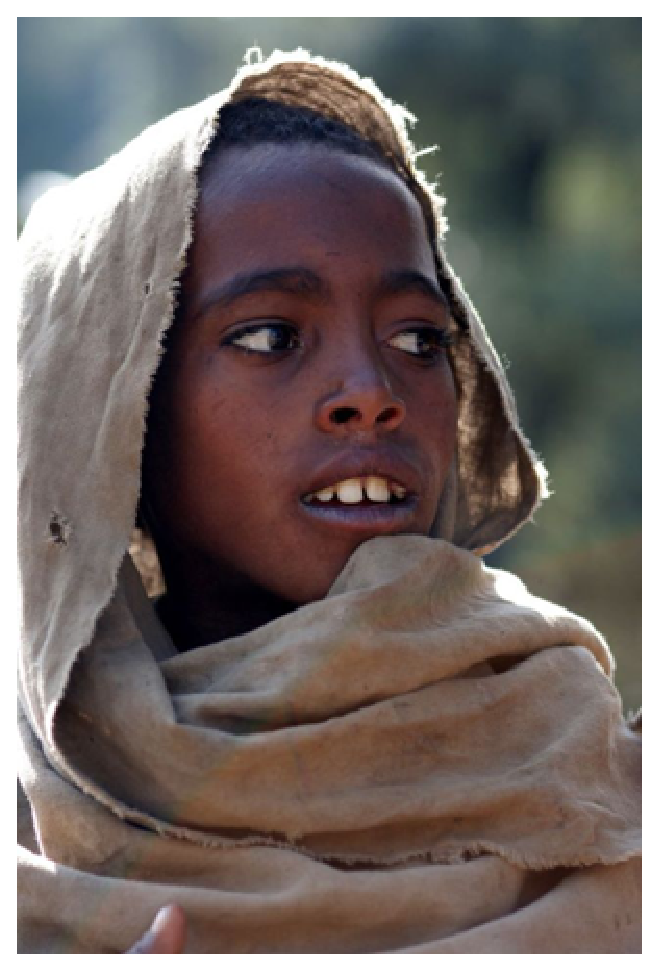
\includegraphics{etiopan.eps}}
	}
\caption{Malý etiopánek a~jeho bratříček}
\label{etiopan}
\end{center}
\end{figure}
\newpage

Rozdíl mezi vektorovým\,\ldots

\begin{figure}[ht]
\begin{center}
{
	
\includegraphics[scale=0.4]{oniisan.eps}
}
\caption{Vektorový obrázek}
\label{oniisan}
\end{center}
\end{figure}

\noindent \,\ldots a bitmapovým obrázkem
\begin{figure}[ht]
\begin{center}
{
	
\includegraphics[scale=0.6]{oniisan2.eps}
}
\caption{Bitmapový obrázek}
\label{oniisan2}
\end{center}
\end{figure}

\noindent 
se projeví například při zvětšení.

Odkazy (nejen ty) na obrázky \ref{etiopan}, \ref{oniisan} a~\ref{oniisan2}, na tabulky \ref{kurzy} a~\ref{tabulky} a~také na algoritmus \ref{algoritmus-1} jsou udělány pomocí křížových odkazů. Pak je ovšem potřeba zdrojový soubor přeložit dvakrát.

Vektorové obrázky lze vytvořit i~přímo v~\LaTeX u, například pomocí prostředí \texttt{picture}. Všechny rozměry jsou uváděny v~mm.

\newpage
% Zaverecny vektorovy obrazek
\begin{figure}
\begin{center}
\setlength{\unitlength}{4pt}
\begin{picture}(115,158.5)
	\put(0,0){\linethickness{1pt}\framebox(115,158.5){}} %ramcek, cely obrazok
	\put(57.5,3){\vector(1,0){57.5}} %Šírka stránky = 115
	\put(57.5,3){\vector(-1,0){57.5}}
	\put(52,3){\makebox (10,5){\shortstack{Šírka stránky = 115}}}
	\put(112,79.25){\vector(0,1){79.25}}
	\put(112,79.25){\vector(0,-1){79.25}}
	\multiput(0,144)(10,0){11}{\line(1,0){7}}
	\multiput(15,151.5)(0,-10){16}{\line(0,1){7}}
	\put(7.5,93){\vector(1,0){7.5}}
	\put(7.5,93){\vector(-1,0){7.5}}
	\put(2.5,93){\makebox (10,5){\shortstack{Mezera = 15}}}
	\put(58,137){\vector(1,0){27.5}}
	\put(58,137){\vector(-1,0){27.5}}
	\put(55,137){\makebox(5,5){\shortstack{Šírka boxu = 55}}}
	\put(30,124){\linethickness{1pt}\framebox(55,10){\textbf{Hlavička}}}
	\put(30.5,35){\linethickness{1pt}\framebox(55,75){\textbf{Textové tělo}}} %telo
	\put(30.5,10){\linethickness{1pt}\framebox(55,10){\textbf{Pata}}}

	\put(88.27,151.25){\vector(0,1){7.25}}
	\put(88.27,151.25){\vector(0,-1){7.25}}
	\put(90.4,144){\makebox(15,15){\shortstack{Výška \\ mezery\,=\,14,5}}}
	\put(88.27,139){\vector(0,1){5}}
	\put(88.27,139){\vector(0,-1){5}}
	\put(89.5,132){\makebox(15,15){\shortstack{Výška \\ mezery\,=\,10}}}
	\put(88.27,129){\vector(0,1){5}}
	\put(88.27,129){\vector(0,-1){5}}
	\put(89.5,122){\makebox(15,15){\shortstack{Výška \\ hlavičky\,=\,10}}}
	\put(88.27,117){\vector(0,1){7}}
	\put(88.27,117){\vector(0,-1){7}}
	\put(89.5,110){\makebox(15,15){\shortstack{Výška \\ mezery\,=\,14}}}
	\put(88.27,72.5){\vector(0,1){37.5}}
	\put(88.27,72.5){\vector(0,-1){37.5}}
	\put(88,57){\makebox(15,15){\shortstack{Výška \\ těla\,=\,75}}}
	\put(88.27,27.5){\vector(0,1){7.5}}
	\put(88.27,27.5){\vector(0,-1){7.5}}
	\put(89.5,19){\makebox(15,15){\shortstack{Výška \\ mezery\,=\,15}}}
	\put(88.27,15){\vector(0,1){5}}
	\put(88.27,15){\vector(0,-1){5}}
	\put(88.5,6.8){\makebox(15,15){\shortstack{Výška \\ paty\,=\,10}}}
	\put(90,93){\vector(-1,0){4.5}}
	\put(90,93){\vector(1,0){4.5}}
	\put(87,98){\makebox(20,15){\shortstack{Mezera\,=\,9}}}
	\put(94,104){\vector(-1,-3){3.65}}
	\put(102,93){\vector(-1,0){7.5}}
	\put(102,93){\vector(1,0){7.5}}
	\put(92,89){\makebox(20,15){\shortstack{Šírka \\ boxu\,=\,15}}}

	\put(94.5,79.25){\linethickness{1pt}\framebox(15,10){\textbf{\shortstack{Okrajová\\ poznámka}}}}
	\put(94.5,43.5){\makebox(15,15){\shortstack{Výška \\ stránky\,=\,158,5}}}
	\put(102,55.5){\vector(1,1){10}}
\end{picture}
\caption{Vektorový obrázek v~prostředí \texttt{picture}}
\end{center}
\end{figure}




\setlength{\unitlength}{2mm}
\begin{picture}(30,20)
\multiput(10,0)(10,0){30}
{\line{1,0}{30}}
\end{picture}

















\end{document}